\subsubsection{Superadditivität}
\label{supadd}
Im folgenden zeigen wir die Superadditivität das CSG. Intuitiv zeigen wir, das ein Spieler immer nur positiven Wert in die Koalition mit einbringt.

\begin{lemma}[Superadditivität]
Das CSG ist superadditiv.
\end{lemma}

Bevor wird die Superadditivität des CSG zeigen, füren wir zunächst zwei weitere ''simple'' Signaturen mit dazugehörigen Modellklassen ein und zeigen, dass Ergebnisse auf ihnen direkt auf CSG übertragen werden können. Außerdem führen wir die Begriffe \textit{potentielle Matches} einer Koalition, die Menge der \textit{gleichzeitig möglichen Baustellen einer Koalition}, \textit{Outcome-Menge} von zwei Koalitionen und den \textit{Wert} einer Baustelle ein:

\begin{enumerate}
  \item \textbf{SCSGS} - Simple Coalition Skill Game Setting
  \item \textbf{SCSG} - Simple Coalition Skill Game
\end{enumerate}

\noindent
Wir zeigen im folgenden, dass sich jedes Setting bzw. Game zu einem Setting bzw. Game vereinfachen lässt, in dem jeder Agent nur eine Einheit eines Skilltypen besitzt. Diese Vereinfachung erleichtert uns den Beweis der Superadditivität und die Betrachtung möglicher Algorithmen zur Verteilungsberechnung. Hierfür benötigen wir jedoch die neue Relation $AgentOwner_{/2}$, mit der wir uns die Zuteilung einer Skillkapazität zu seinem ursprünglichen Agenten merken:

\begin{definition}[SCSGS]
  Eine \textsc{Simple Coalition Skill Game Setting}-Signatur sei definiert als
  \begin{align*}
    \sigma_{SCSGS}:= &\{gentOwner_{2}, Agent_{/1}, Baustelle_{/1}, supply_{/2}, \\
    &demand_{/2}, budget_{/1}, kosten_{/4} \}
  \end{align*}
  \noindent
  \textbf{Intuition} \\
    \begin{tabular}{lrl}
    $AgentOwner(a, x)$&$:\Leftrightarrow$& Agent $x$ gehört zu dem Agenten $a$ \\
    $Agent(x)$&$:\Leftrightarrow$& $x$ ist ein Agent (Baufirma) \\
    $Baustelle(x) $&$:\Leftrightarrow$& $x$ ist eine Baustelle \\
    $type(x)\mapsto t $&$:\Leftrightarrow$& Agent $x$ ist vom Skilltyp $t$ \\
    $demand(x, t)\mapsto n $&$:\Leftrightarrow$& Baustelle $x$ benötigt $n$ Einheiten \\&& vom Skilltyp $t$ \\
    $budget(x)\mapsto n $&$:\Leftrightarrow$&
    Baustelle $x$ zahlt einen Gewinn $n$ \\&& bei Fertigstellung aus\\
    $kosten(t, n, a, y)\mapsto n$&$:\Leftrightarrow$& Kosten für zugehörigen  Agenten $a$ \\&& für die Bereitstellung von $n$ Einheiten \\&& des Skilltyps $t$ an Baustelle $y$
    \end{tabular}
\end{definition}

\noindent
Wir bezeichnen eine $\sigma_{SCSGS}$-Struktur $\mathcal{SS}$ als \textit{Simple Setting} und die dazugehörige Modellklasse valider Strukturen $M_{SCSGS}$. Validitätskritärien sind analog zu $M_{CSGS}$.

\begin{definition}[SCSG]
  Eine \textsc{Simple Coalition Skill Game}-Signatur (SCSG) sei definiert als
  \begin{align*}
    \sigma_{SCSG}:=\sigma_{SCSGS}\cup\{M_{/3}, v_{/2}\}
  \end{align*}
  \noindent
  \textbf{Intuition} \\
    \begin{tabular}{lrl}
    $m(x, t, y)$&$:\Leftrightarrow$& Agent $x$ sendet eine Einheiten des Skilltyps $t$ \\&& an die Baustelle $y$ \\
    $v(x,y)\mapsto n$&$:\Leftrightarrow$& Agent $x$ erhält von Baustelle $y$ die Vergütung $n$
    \end{tabular}
\end{definition}

\noindent
Wir bezeichnen eine $\sigma_{SCSG}$-Struktur $\mathcal{SG}$ als \textit{Simple Game} mit der dazugehörigen validen Modelklasse $M_{SCSG}$. Validitätskriterien sing analog zu $M_{CSG}$.


\subsection{Beziehungen zwischen den Modellklassen}
\label{bez}

Die nachfolgenden Betrachtungen wollen wir jedoch auf einer vereinfachten Strukturen anstellen: Bei  dieser besitzt jeder Agent nur eine Einheit eines Skilltyps. Um dennoch Aussagen über das CSG machen zu können, zeigen wir, dass sich jedes Setting bzw. Game zu einem Simple Setting bzw. Simple Game überführen lässt. Das erlaubt uns die Ergebnisse von  theoretische Betrachtungen von Mechanismen, die bei einem Simple Setting ein Simple Game berechnen, auf das CSG zu beziehen.


\noindent
Formal:
\[
\begin{tikzcd}[column sep=1in,row sep=1in]
M_{CSGS} \arrow{d}{\pi} \arrow{r}{\pi'^{-1}\ \circ\  m'\ \circ\ \pi} & M_{CSG} \\
M_{SCSGS} \arrow{r}{m'} & M_{SCSG} \arrow{u}{\pi'^{-1}}
\end{tikzcd}
\]

\noindent
Dabei müssen folgende Eigenschaften gelten:
\begin{eqnarray}
  \pi &-&\text{total, injektiv} \\
  \pi^{-1}&-&\text{surjektiv} \\
  \pi' &-&\text{total, injektiv} \\
  \pi'^{-1}&-&\text{surjektiv} \\
  \pi^{-1}\circ\pi &=& id_{M_{CSGS}} \\
  \pi'^{-1}\circ\pi' &=& id_{M_{CSG}}
\end{eqnarray}

\noindent
Weiter werden wir nur Mechanismen betrachten die, am Setting keine Änderungen vornehmen, sondern nur Matchings und die Vergütungsverteilung bestimmen. Auf eine ausführliche Definition der gesuchten Funktionen wird hier ebenfalls verzichtet,  stattdessen wird eine Intuition gegeben: Ein Setting bzw. Game lässt sich in ein Simple Setting bzw. Simple Game überführen, indem jede Einheit eines Skilltyps eines Agenten als eigenständiger Agent betrachtet wird.

Dabei wird die Zugehörigkeit von Agenten zum Skill in der $Agent\-Owner$ Relation gesichert. Die Kostenfunktion bleibt bestehen und wird lediglich auf den $AgentOwner$ übertragen. Bei den Matches und Vergütungen wird ähnlich verfahren. Hierdurch gehen keine Informationen verloren und alle Betrachtungen können auf den vereinfachten Modellen durchgeführt werden.



\begin{definition}[Potentielle Matches einer Koalition]
  Sei $K\subseteq Agent$ eine beliebige Koalition. Für $K$ definieren wir die \textit{Menge der potentiellen Matches} $PM(K)$ als

  \begin{eqnarray}
    PM(K) := \{ &\\
    & m: Agent \times Skilltyp \times Baustelle \rightarrow \mathbb{N}\ |\\
    & \phi_{Match}(m) \land \\
    & \quad \quad \forall x\;\forall t\;\forall y: m(x,t, y) > 0 \rightarrow x\in K \quad \quad\} \label{matchown}
  \end{eqnarray}

  Dabei bezeichnet $\phi_{Match}(m)$ die Menge der validen Matches:
  \begin{eqnarray}
    \phi_{Match}(m) := \forall x\; \forall t\; : \left(\;\sum_{y\in Baustelle} m(x,t,y)\;\right)\;\leq \;supply(x,t)
  \end{eqnarray}
  Der Ausdruck (\ref{matchown}) verdeutlicht, dass nur solche Matches für eine Koalition betrachtet werden, deren liefernder Agent auch Teil der Koalition ist.
\end{definition}

\begin{definition}[Gleichzeitig mögliche Baustellen einer Koalition]
  Sei $K\subseteq Agent$ eine beliebige Koalition. Die Menge der möglichen Baustellen, die von $K$ gleichzeitig gebaut werden können -- $B(K)$ -- ist definiert als

  \begin{align}
     B(K) := \{\quad &B_k \subseteq Baustelle\ | \\
     &\exists m\in PM(K), \;\forall b\in B_k, \;\forall t: \\
     &\left(\; \sum_{x\in K}m(x,t,b) \;\right)\geq demand(b, t) \quad\}
  \end{align}

\end{definition}

\noindent
Da wir ein Simple Game betrachten, Können wir o.B.d.A. annehmen, dass eine Agent nur einer Koalition zugeordnet ist:
\begin{equation}
  K\neq S \Rightarrow K\cap S =\emptyset \label{koalitiondisjunct}
\end{equation}

\noindent
Hieraus folgt, dass eine Baustelle in einem Spiel nur von einer Koalition gebaut werden kann, da eine Baustelle pro Spiel nur einmal gebaut wird. Um dies formal festzuhalten, definieren wir im Folgenden die Outcome-Relation:

\begin{definition}[Outcome-Menge zweier Koalitionen]
  Seien $K, S \subseteq Agent$ beliebige Koalitionen. Eine \textit{Outcome-Menge} weist beiden Koalitionen ein Tupel der Baustellen zu, die sie jeweils zur gleichen Zeit bauen können:
\begin{align}
  Outcome(K,S) := \{ \; \;
  &(B_K,B_S)\subseteq Baustelle\times Baustelle\ | \\
  &B_K\in B(K) \land B_S\in B(S)\land B_K\cap B_S =\emptyset \;\;\}
\end{align}
\end{definition}

\noindent
% Zur weiteren Vereinfachung definieren wir noch eine Bewertungsfunktion für eine Menge von Baustellen:
%
% \begin{definition}[Wert einer Baustelle]
%   Sei $B\subseteq Baustelle$ beliebig. Dann ist der \textit{Wert} von $B$ definiert als
%   \begin{equation}
%     v(B):=\sum_{b \in B} \; budget(b)
%   \end{equation}
% \end{definition}
%
% \begin{definition}[erzielbarer Wert zweier Koalitionen]
%   Seien $K, S \subseteq Agent$ beliebige Koalitionen. Der \textit{erzielbare Wert zweier Koalitionen} $K$ und $S$ ist nun definiert als
% \begin{align}
%   v(K) + v(S) := \max_{(B_K, B_S)\in Outcome(K,S)} \;(\;
%   &v(B_K) - \varphi_{kosten}(K, B_K) \;+ \\ &v(B_S) - \varphi_{kosten}(S, B_S) \qquad)
% \end{align}
%
% \noindent
% Die Baustellen, die von einer Koalition gebaut werden, können nicht mehr von einer anderen Koalition gebaut werden. Deshalb müssen wir diese zeitgleich betrachten.
% $\varphi_{kosten}(B,K)$ ist dabei diejenige Funktion, die basierend auf der vorhandenen Kostenfunktion, der Koalition und den Baustellen die Kosten der Koalition für die Bereitstellung aller notwendigen Skills berechnet, um die Baustellen fertig zu stellen.
% \textbf{Bemerkung}: Nach Definition ist das Ergebnis pareto-effizient.
% \end{definition}
%
% \noindent
% Existiert eine Koalition isoliert, lässt sich diese auch isoliert betrachten:
% \begin{definition}
%   Sei $K \subseteq Agent$ eine beliebige Koalition.
%   \begin{equation}
%     v(K) := \max_{B'\in B(K)} \left(\; v(B') - \varphi_{kosten}(B', K) \;\right)
%   \end{equation}
% \end{definition}
%
% \noindent
% Insbesondere gilt dann auch für zwei allein agierende Koalitionen $K, S \subseteq Agent$:
% \begin{equation}
%   v(K\cup S) = \max_{B'\in B(K\cup S)} \left(\; v(B')-\varphi_{kosten}(B', K) \;\right)
% \end{equation}
%
% \noindent
Beachte auch das für einen Outcome zweier Koalitionen eine mögliche Baustellenmenge der potentiellen Baustellen der Vereinigung der Koalitionen existiert die alle Baustellen des separaten Outcomes beinhaltet:
\begin{equation}
  \forall (B_K, B_S)\in Outcome(K,S),\; \exists B'\in B(K\cup S):\; B_K\cup B_S\subseteq B'
\end{equation}

\noindent
Hieraus können wir die Superadditivität des Spiels schließen:
\begin{equation}
  v(K\cup S) \geq v(K) + v(S)
\end{equation}
\begin{flushright}
  \qed
\end{flushright}

\subsubsection{instabilität der Großen Koalition}
\label{instabil}

\begin{lemma}[instabilitiät der Großen Koalition]
  Im allgemeinen Fall ist die große Koalition $K=Agenten$ ist instabil.
\end{lemma}

Beweis durch ein Beispiel:
\begin{figure}
  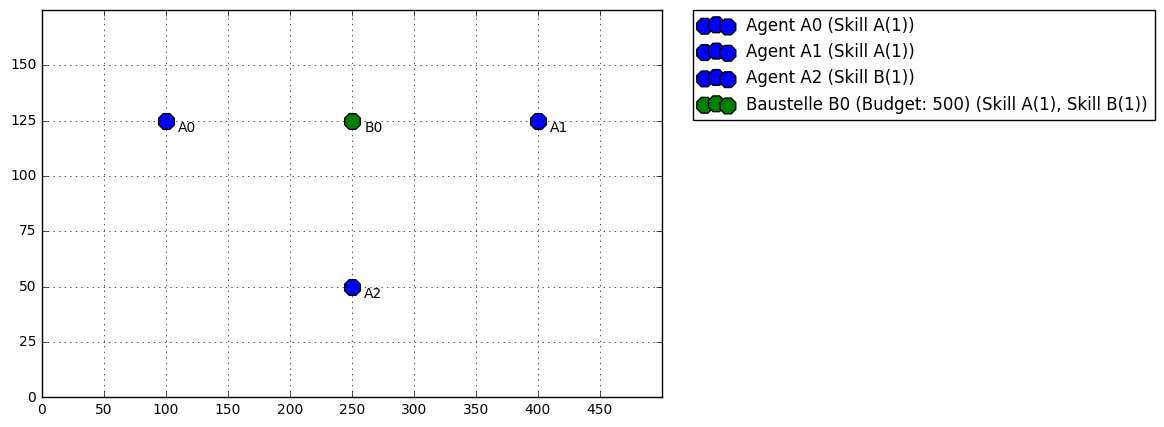
\includegraphics[width=0.5\textwidth]{example-exchangeable-agents.png}
  \caption{Szenario mit einer instabilen großen Koalition.}
  \label{szenario1}
\end{figure}

Im Szenario in Abbildung (\ref{szenario1}) machen die Koalitionen $K_1 = \{A0, A1, A2\}$ sowie $K_2 = \{A0, A2\}$ den gleichen Gewinn, jedoch bekommen die Agenten in $K_2$ Anteilig mehr vom Gewinn. Demnach lohnt es sich für sie die große Koalition zu verlassen.
\begin{flushright}
  $\qed$
\end{flushright}

\subsubsection{NP-härte des Problems}
\label{np}
Im folgenden möchten wir die NP-härte eines gewünschten mechanismusses Zeigen. Hierfür reduzieren wir das Rucksackproblem, ein allgemein bekanntes NP-vollständiges Problem, auf ein CSG.
Das Rucksackproblem ist folgendermaßen definiert:

\begin{lemma}
Sei $m:M_{CSGS}\rightarrow M_{OCSG}$ ein Mechanismus, der ein optimales Matching berechnet, dann ist $m$ NP-hart.
\end{lemma}

\begin{definition}[KNAPSACK]
Sei $U$ eine Menge von Objekten, w eine Gewichtsfunktion und v eine Nutzenfunktion:
\begin{align}
  w: U\rightarrow \mathbb{R} \\
  v: U\rightarrow \mathbb{R}
\end{align}
Sei weiter $B\in\mathbb{R}$ eine vorgegebene Gewichtsschranke.
Gesucht ist eine Teilmenge $K\subseteq U$, die folgende Bedingungen erfüllt:
\begin{align}
  \sum_{w\in K}w(u)\leq B \label{bed1}\\
  max(\sum_{w_in K}v(u)) \label{bed2}
\end{align}
\end{definition}

Sei $K=\{U,w,v\}\in KNAPSACK$ ein beliebiges Rucksackproblem. Wir geben eine übersetzung in eine CSGS-Signatur an:
\begin{align}
  Agent = \{a\} \\
  supply(a, t) \mapsto B \\
  Baustelle = U \\
  demand(u, t) \mapsto w(u) \\
  budget(x) \mapsto v(x) \\
  kosten(t, n, x, y) \mapsto 0
\end{align}
Dabei wird das KNAPSACK problem als ein Spiel mit nur einem Agenten mit einem Skilltyp auf. Die maximale Kapazität des Rucksacks $B$ ist dabei die quantität des Skilltypes des Agenden. Die Menge der Objekte wird als Menge an Bauaufträgen interpretiert, das Gewicht eines Objektes $w(u)$ als die zur fertigstellung geforterten Ressourcen und dessen Wert $v(u)$ das Budget einer Baustelle.

Intuitiv sorgt die Bedingung \ref{bed1} dafür, dass der Agent seine Resourcen nicht überschreitet, sowie die Bedingung \ref{bed2}, dass der Agent sein profiet maximiert. Beides sind ebenfalls Anforderungen, die von einem Mechanismus erfüllt werden müssen der ein optimales CSG berechnet.
Angenommen es gäbe ein $m\in P$ der aus einem CSGS ein CSG mit einem optimalem Matching berechnet, dann währe auch $KNAPSACK\in P$. Dieses ist jedoch ein wiederspruch zur annahme $KNAPSACK\in NP$.
\begin{flushright}
  $\qed$
\end{flushright}

\subsubsection*{Stabilisierung}
\label{stabilisierung}
Wie wir in Abschnit (\ref{instabil}) gesehen haben ist die große Koalition instabil. Im folgenden möchten wir ein Vorschlag zeigen, wie ein Koalitionsbildungsmechanismus funktionieren könnte, der eine stabile große Koalition produziert:
Eine Koalition garantiert ihren Koalitionsteilnehmern beim Beitritt einen individuellen Gewinn in der höhe des Shapley Values und verlangt dafür einen hinreichenden Beitritsdepot $x$. Dieser Kolleteralbetrag wird von einer unabhängigen Instanz verwaltet und Sichert die Agenten vor dem "rauswurf" aus der Großen Koalition ab indem er diese in der gleichen höhe auszahlt, wie auch ihr Gewinn in der Großen Koalition währe. Am Schluss wird der Koleteralbetrag wieder anteilig an die Agenten zurück verteilt. Durch wird die große Koalition Stabilisiert, da es für Teilkoalitionen nicht mehr lohnt auszusteigen, da der Koleteralbetrag um genau den gleichen wert schrumpfen Würde wie die auszahlung der zurückgelassenen Agenten. Der Beitritsdepot für jeden Agenten für die Große Koalition ist $x=\frac{\sum_{b\in Baustellen} budget(b)}{2*|Agenten|}$ (ohne Beweis)

\subsubsection*{Mechanismus}
In Abschnit (\ref{supadd}) sowie (\ref{stabilisierung}) haben wir gezeigt dass der Beitrit zur großen Koalition die rationall richtige entscheidung ist, was die Offenlegung aller Agentenressourcen zur folge hat.
% Da wir aus Abschnit (\ref{np}) wissen das das Berechnen eines optimalen Matchings NP hart ist, können wir entweder, wie im praktischen Teil beschrieben, auf ein Approximationsalgorithmus zurückgreifen oder nach der suche des maximums, alle Möglichen Matchings ausprobieren
Das berechnen eines optimalen Matchings ist entscheidbar, jedoch wie wir aus Abschnit (\ref{np}) wissen, NP-hart.
Das Berechnen des Shapley-Values ist ebenfalls entscheidbar, jedoch ebenfalls NP-hard.
Jedoch haben wir in diesem Kapitel gezeigt, dass es ein NP-harten Mechanismus gibt der gegeben einem Setting ein Faires und Optimales Ergebniss berechnet, welches allen Anforderungen der Aufgabenstellung gerecht wird.
\TODO{referenz auf kritärien der Aufgabenstellung}
